\documentclass[10pt,a4paper]{article}
\usepackage[utf8]{inputenc}
\usepackage{amsmath}
\usepackage{amsfonts}
\usepackage{amssymb}
\usepackage{graphicx}
\usepackage[margin=0.5in]{geometry}

\author{Oleg Loshkin}
\title{\textbf{CSC}\\Convertible Scene Creator\\\textbf{User Manual}}
\graphicspath{{./images/}}

\begin{document}

\maketitle

\section{Introduction}
The \textbf{Convertible Scene Creator, or CSC for short,} is a Unity tool used to \textbf{create .asset ScriptableObjects files from .unity Scenes} for conversion by UPDC.
These .asset files can then be \textbf{used by the Unity to PokEngine Data Converter (UPDC)} to generate .pokconvertiblescene files readable by the PokEngine parser.

\section{Accessing the Tool}
\begin{center}
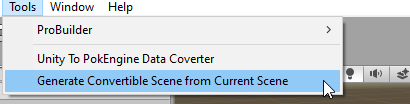
\includegraphics[scale=1.0]{mainMenu}
\end{center}

\section{UI}
\begin{center}
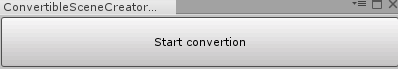
\includegraphics[scale=1.0]{editorUi}
\end{center}
The tool has only one button that when pressed will \textbf{launch the generation} of a .asset file \textbf{for the current scene}. \textbf{The generation may take some time}. Upon completion, the editor will close automatically.

\section{Output File Location}
\begin{center}
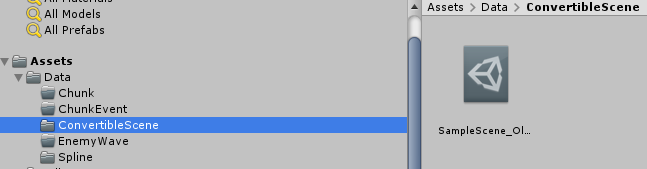
\includegraphics[scale=0.75]{outputFile}
\end{center}
\newpage

\section{Adding a new Convertible Component}
\textbf{CSC allows you to implement the exportation of components it finds on the GameObjects} in the Scene. \textbf{To implement} the exportation of a new component we will name "MyComponent" for example's sake \textbf{you must}:
\begin{itemize}
\item \textbf{Create a new .cs file under "Assets/Editor/CSC/Components"} that will define the convertible component:
\begin{center}
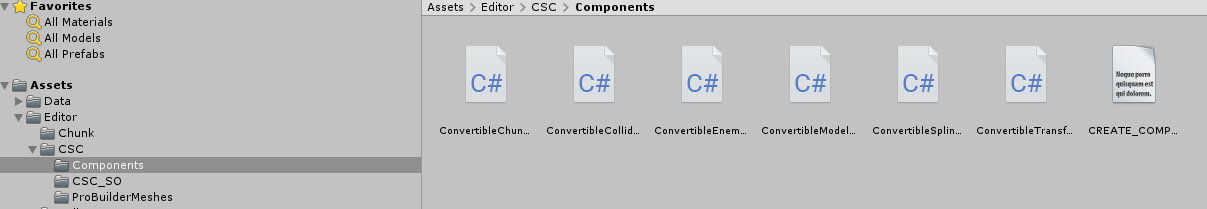
\includegraphics[scale=0.5]{newComponentLocation}
\end{center}
\item \textbf{Inside, you must define the struct that will be serialized}. \textbf{It must be marked as "[System.Serializable]" and must inherit from ConvertibleComponent}.\\
\textbf{Inside, you must also define a creator} for your ConvertibleComponent. \textbf{It must implement a "CreateConvertibleComponents()" method}. See the image below.
\begin{center}
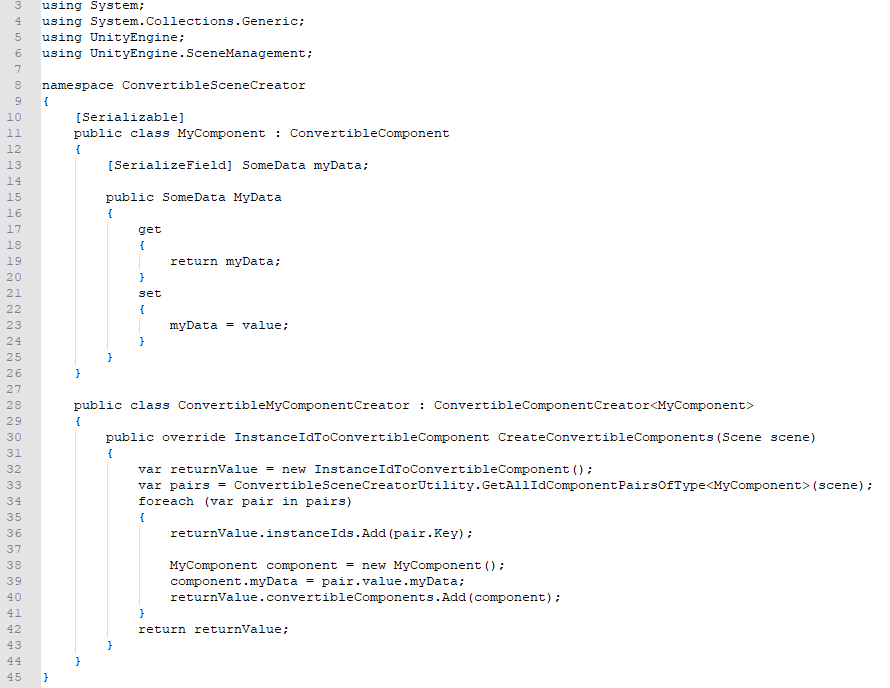
\includegraphics[scale=0.75]{newComponentDeclaration}
\end{center}
See implementations of existing ConvertibleComponents for more examples of implementations.
\newpage
\item Next, \textbf{edit the "Components.cs" file} located under "Assets/Editor/CSC":
\begin{center}
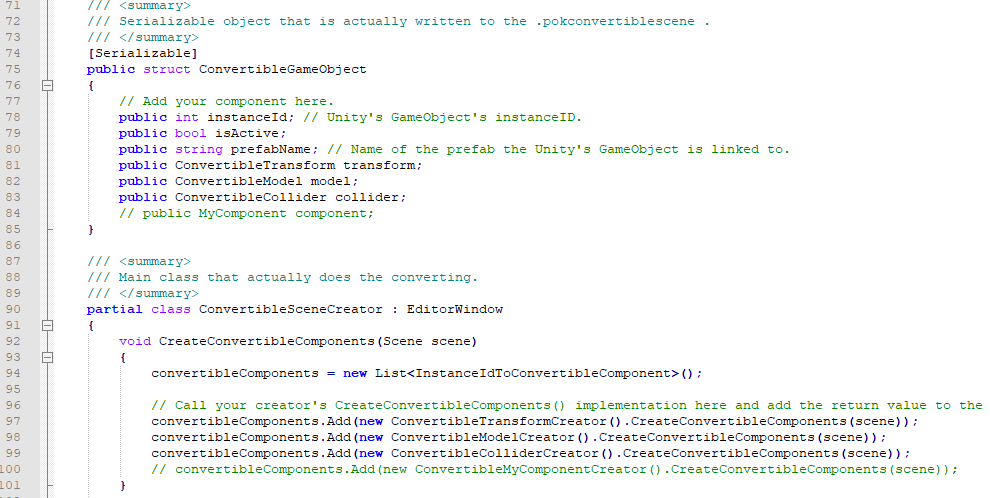
\includegraphics[scale=0.65]{componentsContents0}
\end{center}
Here, you will \textbf{add your new ConvertibleComponent to the declaration of a ConvertibleGameObject}. You will then \textbf{add a line to ConvertibleSceneCreator's CreateConvertibleComponents() method to add the components to ConvertibleSceneCreator's components list.}\\\\
Finally, \textbf{assign your MyComponent to the ConvertibleGameObject by adding a few lines to ConvertibleSceneCreator's GenerateConvertibleGameObject() method} like demonstrated below:
\begin{center}
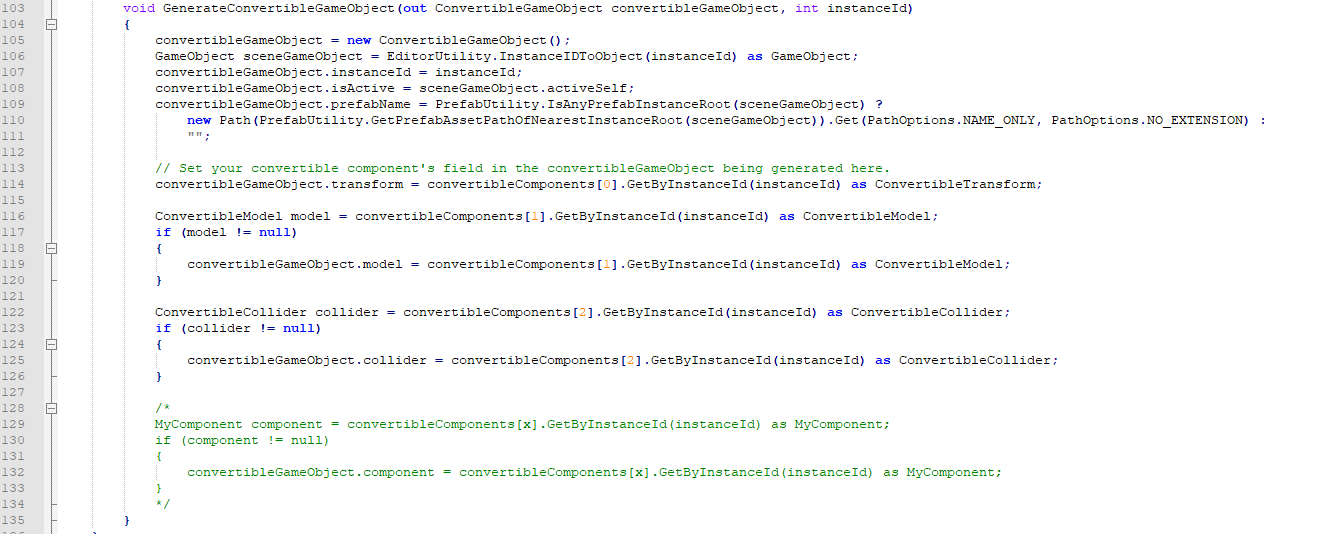
\includegraphics[scale=0.55]{componentsContents1}
\end{center}
\newpage
\item You will also \textbf{need to add a string to UPDC's "Empty Fields" tab that defines what an empty MyComponent looks like in JSON format}. This will make sure that the output file will not contain any empty instances of your new component.
\begin{center}
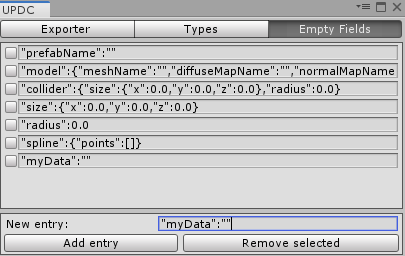
\includegraphics[scale=1.0]{emptyDefinition}
\end{center}
\end{itemize}
You should now be able to see the values of your new component in any new .asset file's inspector and upon exporting it, the resulting JSON file should not have any uninitialized instances of your component.

\end{document}
